\chapter{Process Overview}\label{Ch2}

Pad manufacturing is a complex and intricate process that encompasses multiple stages, from the selection of raw materials to the final packaging of the pads. Each stage involves specialized machinery, precise measurements, and stringent quality control measures to ensure the production of safe, comfortable, and hygienic products. 

The Ultra Pads manufacturing at P\&G Crailsheim is carried out by lines $13$, $15$, $16$, $19$, $20$, $21$, and $22$. The manufacturing process begins with the Top and the Second-Top Sheets, both materials come as rolls that are placed by a robot in the Unwind UNW Module. In this module, the rolls are rotating at a specified speed, and with the use of Idler-Rolls the web is fed into the Line; the rolls act supported by a Fife Sensor to control the tension and the position of the Web in the Machine-Direction (MD) and Cross-Direction (CD). Both materials run independently through the DPM, where the design pattern is printed on the TS.

The STS continues till it enters the STS C\&L where is cut according to the production format, then it is placed over the TS so they can be bonded together on the Fusion Bond Unit ((FSB) and continue to run as a unique material web before the Core is placed on the Core Cut-and-Slip (CCS); for the core placement a special glue (AWA) is used, it is followed by the Scent application on the ONM Module. 

At this point, the Pad lacks the Backsheet (BS) which is placed and fixed to the other material layers via the Crimper Module; the BS is the layer that comes in contact with the underwear, therefore a special glue (WLA) is spread on it. Both types of glue are applied at a high temperature, to cool them down, the web passes through two cooled rolls placed on the Activation Chamber (ACT). Finally, the web enters the Final Knife (FNK) where it is cut according to the format, and the Pad Wings are obtained.

After this, the Pad is already manufactured and the remaining stages of the process focus themselves on the folding and packaging of each Pad for the finished product. These processes exceed the Scope of this study.

%The Lines Layout and Process Descriptions were taken from~\cite{layout}.
%%--------------------------------------------------------------------------%%

\section{The STS C\&L Module}\label{sec2.1}

This module is placed between the DPM and the FSB, it is the first part of the process in which the TS and the STS (colored green and blue in Figure~\ref{flow} respectively)  interact with one another. The STS enters the Module from the Ceiling via the infeed conveyor (number 1 in Figure~\ref{flow}), the material enters as a continuous web and is cut inside at a specific length. Inside the module (number 2 in Figure~\ref{flow}) there are two rollers, the anvil roll helps the web to travel through the module and presses it against the knife, then it is cut to the required length and in the desired shape, the remaining pieces are thrown away via the Chute Vacuum that is placed under the STS C\&L (number 3 in Figure~\ref{flow}), the cut STS  and its transfer to the Lay-Down-Drum (also known as Transfer-Drum, marked as 4 in Figure~\ref{flow}).

From this point, it is placed over the TS and transported to the FSB as a single web (colored as violet in Figure~\ref{flow}). 

%The STS C\&L complete assembly and additional actuators are shown in Figure~\ref{Module}. 

\begin{figure}[H]
    \centering
    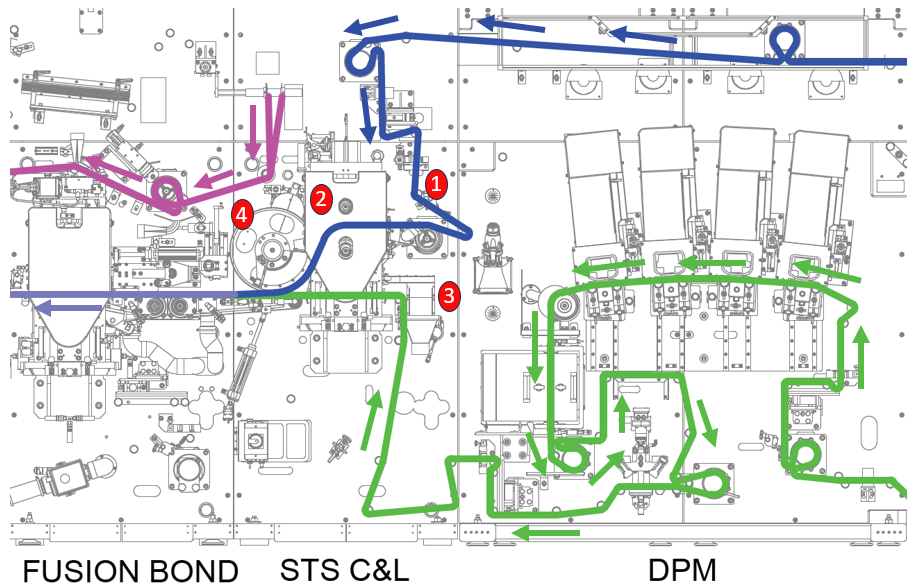
\includegraphics[width=1\linewidth]{FIGURES/flow.png}
    \caption{TS and STS Work Path through STS C\&L Module~\cite{layout}.}
    \label{flow}
\end{figure}


%\begin{figure}[H]
 %   \centering
  %  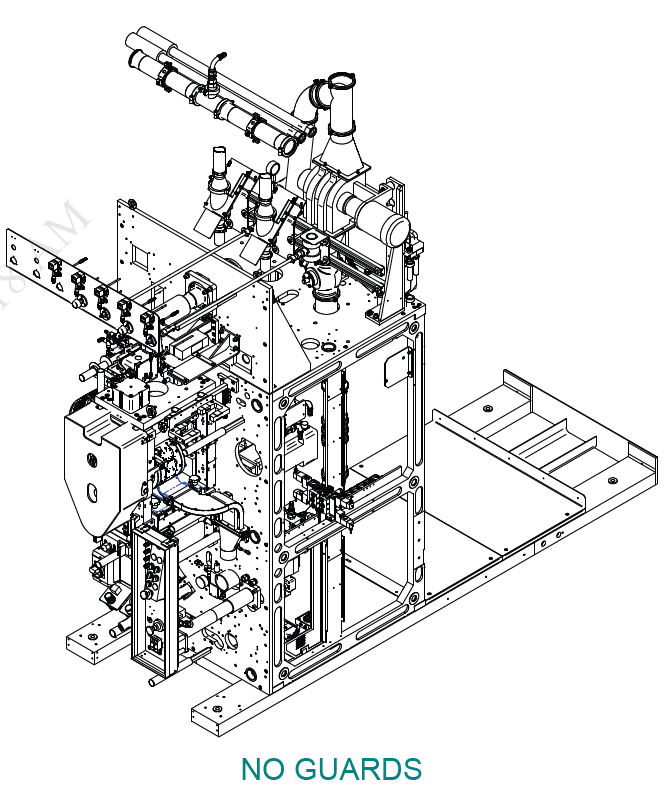
\includegraphics[width=0.5\linewidth]{FIGURES/STSModule.png}
   % \caption{Drawing of the STS C\&L Module without Guards~\cite{module}.}
    %\label{Module}
%\end{figure}
%\begin{figure}[!tbp]
%  \begin{subfigure}[b]{0.5\textwidth}
%    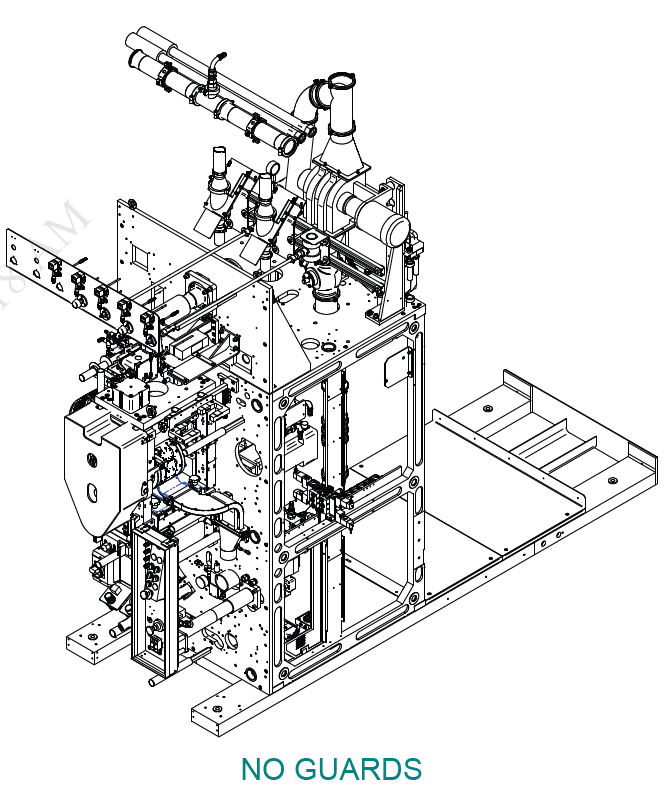
\includegraphics[width=\textwidth]{FIGURES/STSModule.png}
%    \caption{Isometric View.}
    %\label{fig:f1}
%  \end{subfigure}
%  \hspace{2cm}
%  \begin{subfigure}[b]{0.3\textwidth}
%    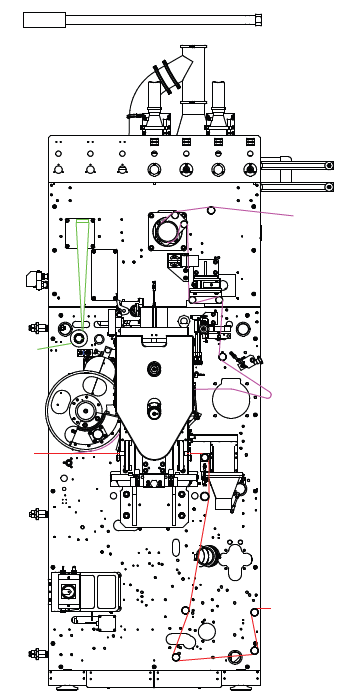
\includegraphics[width=\textwidth]{FIGURES/STSModule2.png}
%    \caption{Front View.}
    %\label{fig:f2}
%  \end{subfigure}
%  \caption{Drawing of the STS C\&L Module without Guards~\cite{module}.}
%  \label{Module}
%\end{figure}

%%----------------------------------------------------------------%%
\subsection{The Knife Roll}\label{sec2.1.1}

%Although each pad size employs a different cutting unit, the working principle is the same for all, and the operating conditions do not differ greatly, the average working pressure of the units is $4$~bar

Inside the STS C\&L Unit are two parallel rollers: the anvil roll, responsible for helping the web pass through the module and pressing it against the knife roll, this one is located under the anvil and is accountable for cutting the STS in their different formats. 

The knife roll is mounted over a shaft that rotates due to an electric motor placed on the Drive Side (DS) of the Line, the web is cut due to the pressure imposed by the anvil over the knife. To make sure that the web is held correctly, the knife roll has little holes inside and outside the pad print, these holes suck in air and hold the web in position, as well as the remaining parts of the web that are thrown away after cutting.

Figures~\ref{knife} and~\ref{knife2} show the knife roll a complete view of the knife roll assembly in the STS C\&L unit and an isolated view of the roll itself respectively. 

\begin{figure}[H]
    \centering
    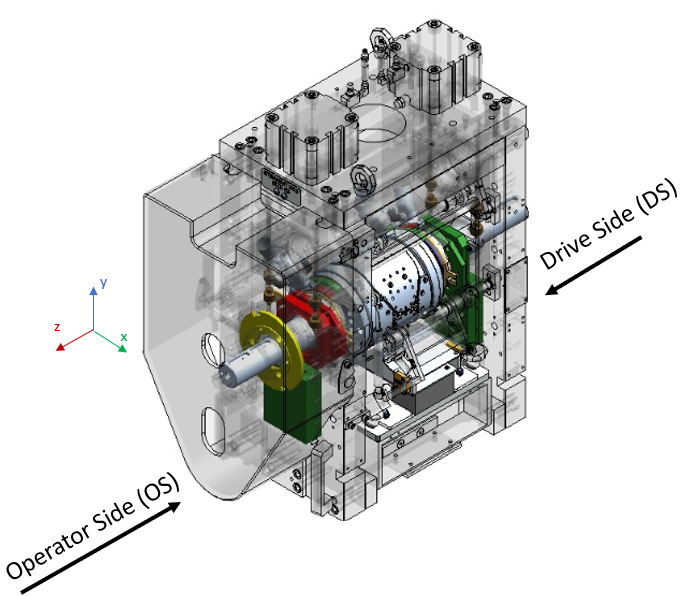
\includegraphics[width=1\linewidth]{FIGURES/knife.png}
    \caption{Assembled Knife Roll of STS C\&L Unit~\cite{knife}}
    \label{knife}
\end{figure}

\begin{figure}[H]
\centering
  \begin{subfigure}{0.35\textwidth}
  \centering
    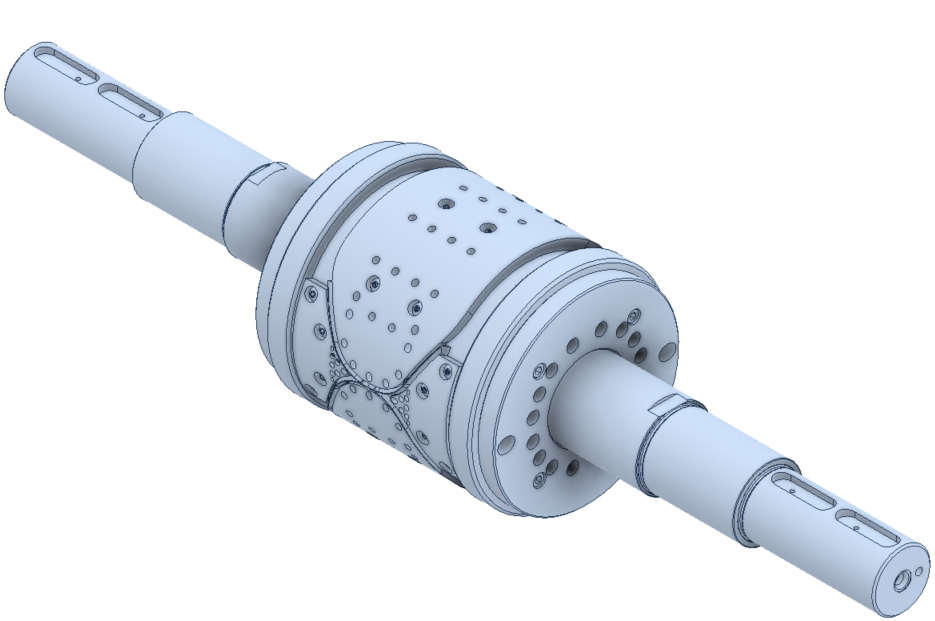
\includegraphics[width=1.1\linewidth]{FIGURES/knife1.png}
    \caption{Isometric View.}
  \end{subfigure}
  %\hspace{1cm}
  \begin{subfigure}{0.3\textwidth}
  \centering
    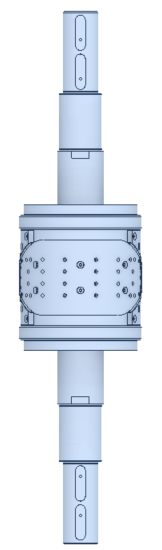
\includegraphics[width=0.5\linewidth]{FIGURES/knife2.png}
    \caption{Top View.}
  \end{subfigure}
  %\hspace{1cm}
  \begin{subfigure}{0.3\textwidth}
  \centering
    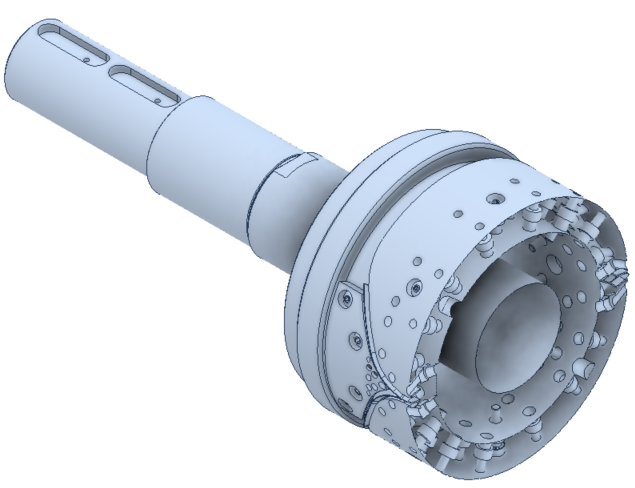
\includegraphics[width=1.1\linewidth]{FIGURES/knife3.png}
    \caption{Half-Section View.}
  \end{subfigure}
  \caption{Drawing of the Knife Roll~\cite{knife}.}
  \label{knife2}
\end{figure}
%\clearpage
%%---------------------------------------------------------------%%
\subsection{The Vacuum Manifold}\label{sec2.1.2}

The suction power that allows the knife roller to hold the web comes from the vacuum manifolds. Every unit has two manifolds located at each side of the knife roll (OS and DS), both manifolds are connected directly to the main air system. Figure~\ref{knife&manifold} shows both manifolds assembled to the knife roll. 
\begin{figure}[H]
    \centering
    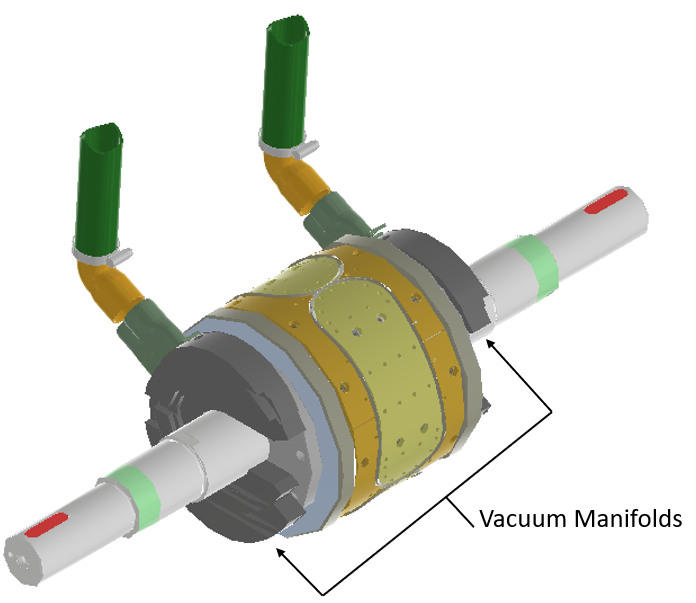
\includegraphics[width=0.65\linewidth]{FIGURES/manifold1.png}
    \caption{Vacuum Manifolds Assembled with Knife~[Author].}
    \label{knife&manifold}
\end{figure}

The manifolds are responsible for holding the STS web once it is cut in the required shape (pad vacuum), for holding the remaining web pieces after the cut is done (trim vacuum), for blowing air so that the shaped web can be transferred to the Transfer Drum (pad blow-off), and for blowing the remaining pieces into the chute vacuum (trim blow-off). This is achieved through the different air chambers inside the manifold marked in Figure~\ref{manifolds}.
\begin{figure}[H]
\centering
  \begin{subfigure}{0.4\textwidth}
  \centering
    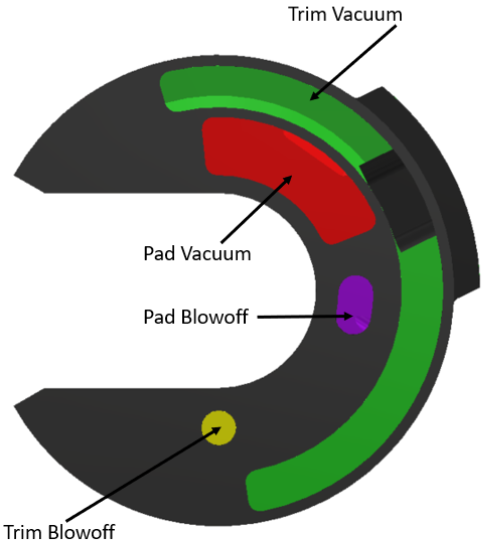
\includegraphics[width=0.8\linewidth]{FIGURES/manifoldOS.png}
    \caption{Vacuum Manifold OS.}
  \end{subfigure}
  %\hspace{1cm}
  \begin{subfigure}{0.4\textwidth}
  \centering
    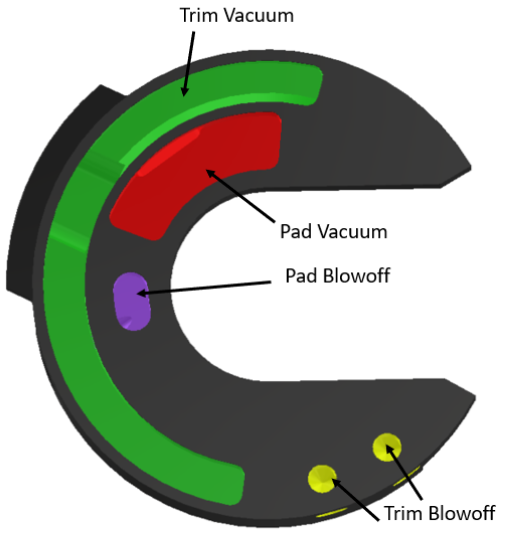
\includegraphics[width=0.8\linewidth]{FIGURES/manifoldDS.png}
    \caption{Vacuum Manifold DS.}
  \end{subfigure}
  \caption{Air Chambers of the Vacuum Manifolds~[Auhtor].}
    \label{manifolds}
\end{figure}

%%----------------------------------------------------------%%
\subsection{The Transfer Drum}\label{sec2.1.3}

After the knife roll has cut the STS, it has to be placed over the TS so that the manufacturing can continue. This is done via the Transfer Drum, which holds the pad that has been blown from the cutting unit and gently places it over the TS that has been traveling in the conveyor.

The drum consists of a cylinder that is rotating opposite to the knife roll, inside it there is a vacuum manifold with two air outlets, one placed at the top and one at the bottom) and provide the suction power to hold the pad until it is placed on the conveyor; for the biggest formats, an accessory called the Blow-Off can be added to the drum, it is used to blow air to the STS once is placed over the TS to assure that they are in full contact. Figure~\ref{drum} shows the transfer drum with its main components and the blow-off air accessory.

\begin{figure}[H]
    \centering
    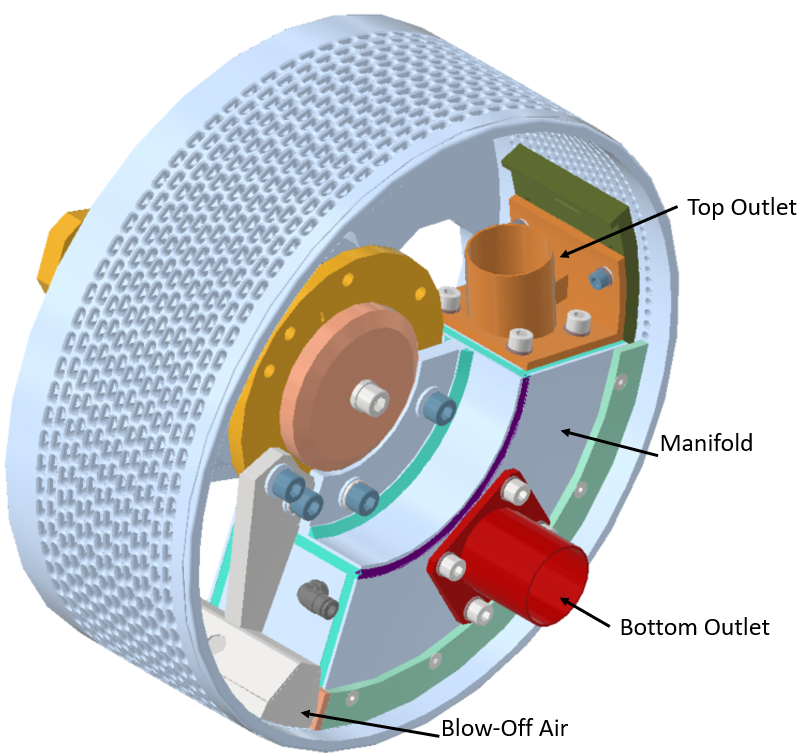
\includegraphics[width=0.5\linewidth]{FIGURES/drum.png}
    \caption{Transfer Drum with Components and Blow-Off Air~[Author].}
    \label{drum}
\end{figure}

Once the STS is laid over the TS, they leave the STS C\&L and continue to the FSB unit, in this unit, an embosser (BOE) presses both materials together to connect them without using any glue: The Bonding has the appearance of the little holes shown in Figure~\ref{fsb}.
\begin{figure}[H]
    \centering
    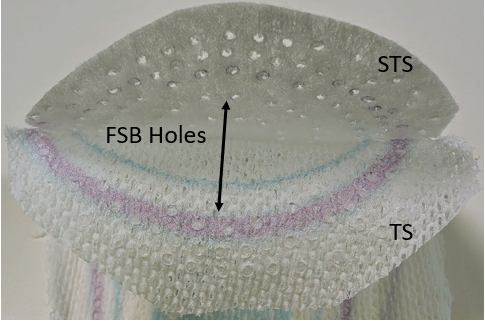
\includegraphics[width=0.8\linewidth]{FIGURES/fsb.png}
    \caption{Bonded TS and STS~[Author].}
    \label{fsb}
\end{figure}
\clearpage
%%------------------------------------------------------------------------%%
\section{Parameters Monitoring}\label{sec2.2}

The Touchless Quality Team of P\&G main goal is to enhance and streamline the quality management processes by leveraging automation, digital technologies, and data-driven approaches. Thus, they have invested in sensors and data acquisition systems to track important operation parameters and variables that influence directly the overall manufacturing processes of all lines.  

The collected data is monitored using Grafana, which is an open-source data visualization and monitoring tool that facilitates the creation of interactive dashboards and charts for analyzing and monitoring diverse data sources. It supports a broad range of data sources, including databases, time series databases, cloud services, etc. 

Grafana can establish connections with various data sources, these data sources serve as repositories for the data that users intend to visualize or monitor. With the data in the repositories, different Dashboards can be created to provide a web-based interface that enables users to create and configure dashboards. Dashboards are composed of panels that display visualizations (tables, graphs, etc.). The data can also be downloaded for future analysis and post-processing. 

An example of one of the created dashboards tracking the caliper of a pad is shown in Figure~\ref{dashboard1}, the left $y$-axis shows the caliper in [mm], and the $x$-axis shows the time.

\begin{figure}[H]
    \centering
    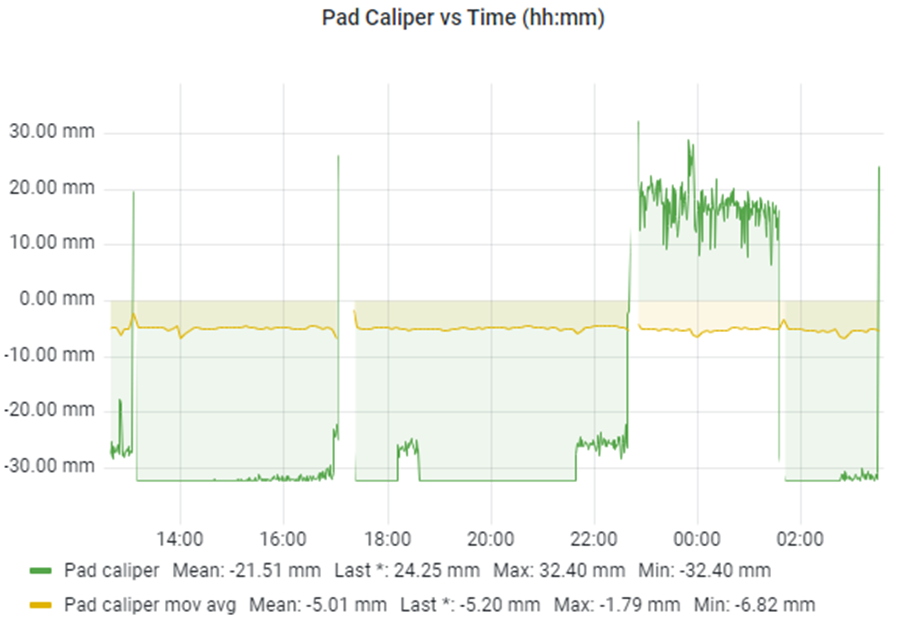
\includegraphics[width=1\linewidth, height=0.35\textheight]{FIGURES/dashb1.png}
    \caption{Pad Caliper Sensor from L19~[Author].}
    \label{dashboard1}
\end{figure}
%%-----------------------------------------------------------%%
\section{Correlation Anaylisis of STS C\&L Parameters}

By exploring the correlations, valuable insights can be gained into the interdependencies and patterns within the STS C\&L parameters, providing a deeper understanding of their behavior and potential impacts. This analysis can potentially uncover meaningful associations and enhance decision-making processes related to STS C\&L. All the Lines mentioned in Chapter~\ref{Ch2} were monitored for 15 days.

Special interest was in the vacuum, the web (width, caliper, CD and MD placement), and unit pressure parameters. This decision was made based on feedback from the different operators at each line. For this purpose, the "STS Foldback Analysis" dashboard was used, the Figure~\ref{STSanalysis} shows the \textit{STS Foldback Rejections} on the right $y$-axis and the \textit{SCL Transfer Drum Vacuum} in [mBar] on the left $y$-axis, the $x$-axis corresponds to the time. The other tracked variables on the PLC are listed above the graph.

The data plotted in the dashboard was downloaded on a CSV file to perform a correlation analysis, the results show that the parameters with the highest correlation to the \textit{STS Foldback Rejections} are those related to the vacuum system of the line, for the \textit{ RTT scl blow off}, \textit{Proportional valves pad blow off}, and the \textit{Trim set point} the correlation coefficient is undefined and showed as NaN, this occurs because most of the registered points for these variables are $0$ and the calculation cannot be done. Figure~\ref{corr} presents the complete correlation matrix as a heat map.

\begin{figure}[H]
    \centering
    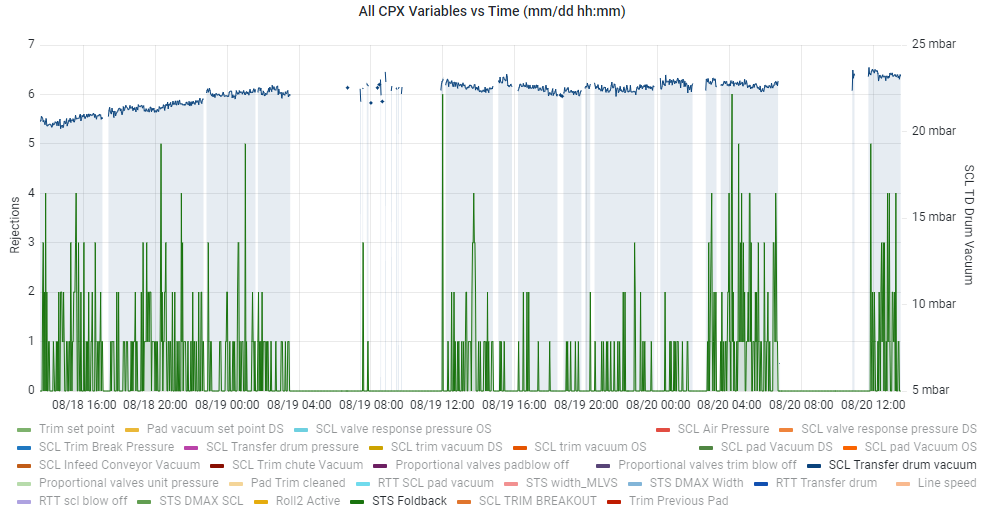
\includegraphics[width=1\linewidth, height = 0.3\textheight]{FIGURES/STSAnalysis1.png}
    \caption{STS Foldback Analysis Dashboard of L19 during the last 30 days~[Author].}
    \label{STSanalysis}
\end{figure}
\begin{figure}[H]
    \centering
    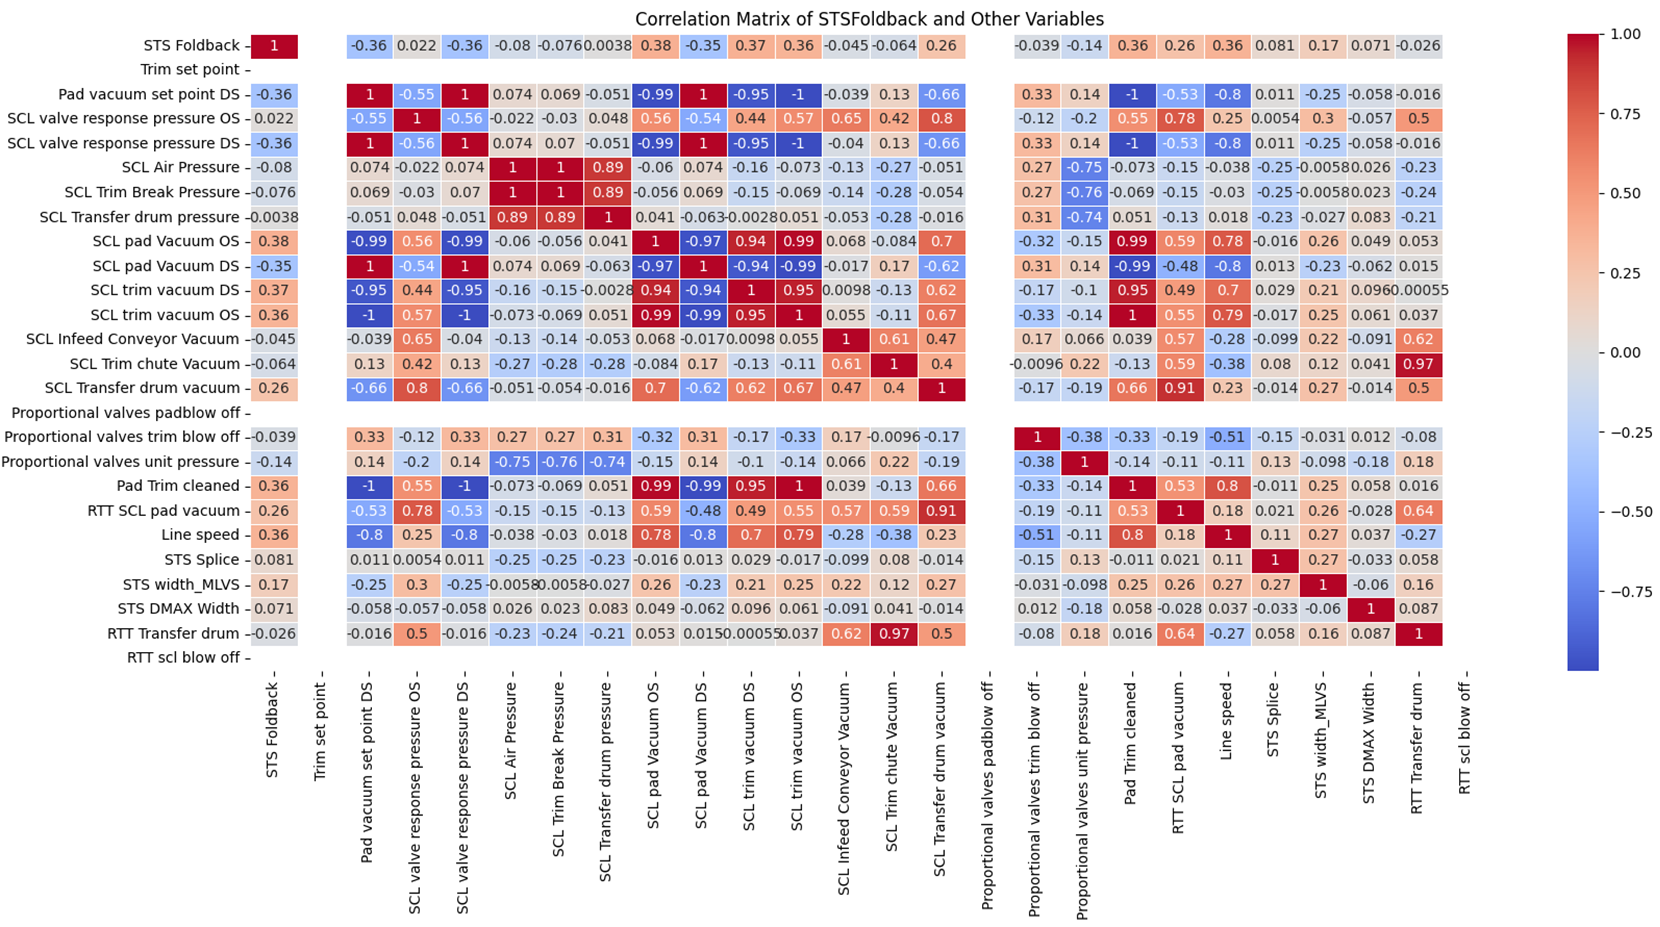
\includegraphics[width=1\linewidth, height = 0.55\textheight]{FIGURES/heatmap.png}
    \caption{Correlation Heatmap~[Author].}
    \label{corr}
\end{figure}
%\clearpage
%%-------------------------------------------------------------------------%%
\section{The Foldback Rejection}

Web foldover also known as foldback, web wrinkling, or buckling are complex and interconnected phenomena that significantly impact continuous manufacturing processes, particularly in industries dealing with thin, flexible materials. These issues are prevalent in sectors such as paper production, textile manufacturing, and thin film fabrication, where maintaining material integrity and quality is paramount~\cite{rosiumconference}.

These phenomena stem from intricate interactions between the web material - typically a continuous sheet or film - and the processing equipment used in its manufacture or handling. The delicate balance of forces acting on the web, including tension, compression, and shear stresses, can be easily disrupted, leading to various forms of deformation.
Web foldover or foldback occurs when the edge of the web material folds onto itself, creating a double-thickness area. Wrinkling, on the other hand, manifests as a series of out-of-plane deformations across the web surface, often resembling waves or ripples. Web buckling represents a more severe form of deformation, where the web experiences a sudden and significant out-of-plane displacement, potentially leading to permanent damage~\cite{Gehlbach1987WebWE}. 

In addition, while transported through the production line, if different sections of the web slip at varying rates, it can create speed differentials across the web width, these differentials can induce shear stresses as the web slips, causing it to break or wrinkle, it also may generate increased friction at certain points, leading to localized heating and potential material deformation. 

The consequences of these phenomena extend beyond mere aesthetic concerns. They can lead to:
\begin{enumerate}
    \item Reduced product quality and increased rejection rates.
    \item Inefficient material utilization and higher scrap rates.
    \item Increased downtime for equipment adjustments and cleaning.
    \item Potential damage to processing equipment.
    \item Inconsistent performance of the final product.
\end{enumerate}

Figure~\ref{foldback2} shows different pads from Line 15 that were rejected due to foldover error. The pads labeled \textit{a, b, e} exhibit a wrinkling foldover, whereas the remaining are completely folded on themselves.
\begin{figure}[H]
    \centering
    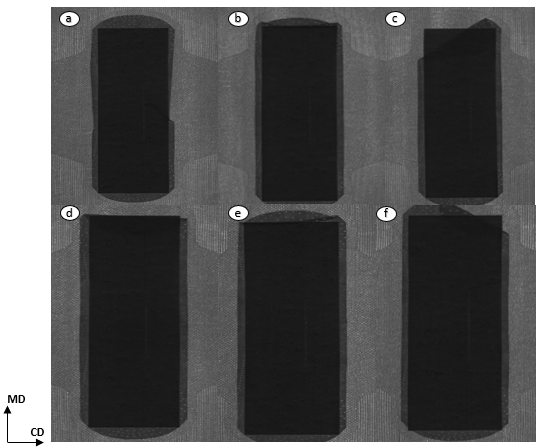
\includegraphics[width=0.75\linewidth]{FIGURES/foldback2.png}
    \caption{Line 15 Pads rejected due to STS Foldback~[Author].}
    \label{foldback2}
\end{figure}

Even though web foldovers are displayed in diverse ways, it is listed under a single rejection cause independently of whether it corresponds to a wrinkling, a buckling, or a complete foldover. The scrap percentage of all the Ultra Lines at P\&G Werk Crailsheim in the last 6 months are shown in Table~\ref{scrap}.

\begin{table}[H]
\centering
\resizebox{\textwidth}{!}{%
\begin{tabular}{cccccccc}
\hline
\textbf{Line} &
  \textbf{Rejection Cause} &
  \textbf{Jan-24} &
  \textbf{Feb-24} &
  \textbf{Mar-24} &
  \textbf{Apr-24} &
  \textbf{May-24} &
  \textbf{Jun-24} \\ \hline
L13 & \textbf{8432 \#64\_UFBVS\_ML\_STS FOLDOVER / WIDTH}  & 0.08\% & 0.15\% & 0.14\% & 0.07\% & 0.12\% & 0.02\% \\
L15 & \textbf{8432-\#064\_UFBVS\_ML\_STS FOLDOVER / WIDTH} & 0.20\% & 0.30\% & 0.23\% & 0.32\% & 0.39\% & 0.33\% \\
L16 & \textbf{8432-\#064\_UFBVS\_ML\_STS FOLDOVER / WIDTH} & 0.54\% & 0.61\% & 0.40\% & 0.46\% & 0.80\% & 0.44\% \\
L19 & \textbf{8432-\#064\_UFBVS\_ML\_STS FOLDOVER / WIDTH} & 0.21\% & 0.44\% & 0.49\% & 0.36\% & 0.13\% & 0.16\% \\
L20 & \textbf{8432-\#064\_UFBVS\_ML\_STS FOLDOVER / WIDTH} & 0.33\% & 0.45\% & 0.41\% & 0.18\% & 0.36\% & 0.52\% \\
L21 & \textbf{8432-\#064\_UFBVS\_ML\_STS FOLDOVER / WIDTH} & 0.11\% & 0.13\% & 0.24\% & 0.15\% & 0.11\% & 0.14\% \\
L22 & \textbf{8432-\#064\_UFBVS\_ML\_STS FOLDOVER / WIDTH} & 0.43\% & 0.47\% & 0.49\% & 0.36\% & 0.52\% & 0.36\% \\ \hline
\end{tabular}%
}
\caption{Scrap Benchmarking Levels in Ultra Lines P\&G Werk Crailsheim~[Author].}
\label{scrap}
\end{table}

%%-------------------------------------------------------------------------%%
\section{Line Selection}

The results from Table ~\ref{scrap} showed that Line 13 has the best scrap level from all the ultra lines, thus choosing it for the implementations could negatively impact the actual production rate. Meanwhile, Lines 16 and 20 show the worst scrap rates from all the Lines, so the impact of the implementations may be more noticeable on them. 

Nevertheless, due to some decisions taken by the Global Leadership Pillar based on the Global Market situation, Line 20 has been producing different formats that normally do not correspond to their main product, as they have held account for some volume losses. 

Therefore, all the implementations and tests described in the upcoming chapters were carried out on Line 16 (the main Line), and Lines 19 and 15.